\section{Problema biológico}

La biología, y en particular la genética, han tenido un lugar destacado en el siglo XX gracias a enormes avances como ser el descubrimiento de la estructura molecular del ADN, con el aporte de Franklin, Crick y Watson \cite{WATSON1953}. A partir de esos hitos científicos, se sucedieron grandes esfuerzos a nivel internacional, como el Proyecto Genoma Humano \cite{Consortium2001} o ENCODE \cite{Consortium2012}, que tienen como objetivo general el mapeo entre código genético humano y sus elementos funcionales. Estos trabajos, sumados a los recientes avances en las tecnologías de secuenciación masiva, han generado un creciente volumen de datos genómicos que a su vez favorecieron la aparición nuevos tipos de tratamientos en el área de la medicina personalizada \cite{doi:10.1056/NEJMp1006304}. 

La medicina personalizada o de precisión es un modelo médico en donde las intervenciones se realizan a individuos o a grupos en riesgo a diferencia del modelo tradicional que apunta a la población en general. \textbf{Dentro de este área, uno de los objetivos críticos que se busca resolver es la detección de variaciones genéticas que deriven en enfermedades}.

\subsubsection{El dogma central de la biología}

El genoma humano esta compuesto por el ADN (ácido desoxirribonucleico), en los 23 pares de cromosomas (moléculas de ADN), dentro del núcleo celular sumado a una molécula de ADN que se encuentra en las mitocondrias (ADN mitocondrial). El ADN a su vez se compone de 4 bases: Adenina, Timina, Citosina, y Guanina. Estas bases se representan con su letra inicial (A, T, C y G), y podemos considerarlas como letras de un alfabeto. Cada una de estas bases está unido a otra (Adenina-Timina y Citosina-Guanina) formando pares de bases en forma helicoidal. Esta tira de ``letras'' se divide en distintos genes, que son secuencias de ADN que codifican una molécula funcional.

Para entender un poco como funciona el proceso por el cual la información genética se expresa en el organismo recurrimos al llamado "Dogma central de la biología", esbozado por Francis Crick en 1958 y revisado en 1970 \cite{CRICK1970}. Este dogma, si bien fue ampliado a lo largo del tiempo, explica de forma general este proceso. Como vemos en la figura, el ADN (ácido desoxirribonucleico) se transcribe en forma de ARN para luego formar una proteína. El ARN (ácido ribonucleico), es una mólecula polimérica, al igual que el ADN, y también posee las mismas bases que el ADN, excepto la timina (T) que se reemplaza por el uracilo (U). Finalmente, el ARN es utilizado para unir los aminoácidos que forman la secuencia proteica, en un proceso denominado Traducción. La secuencia del ARN se compone de tripletes adyacentes de bases que se denominan codones, y cada aminoácido está codificado por uno de estos codones. 

\begin{figure}[H]
\centering
    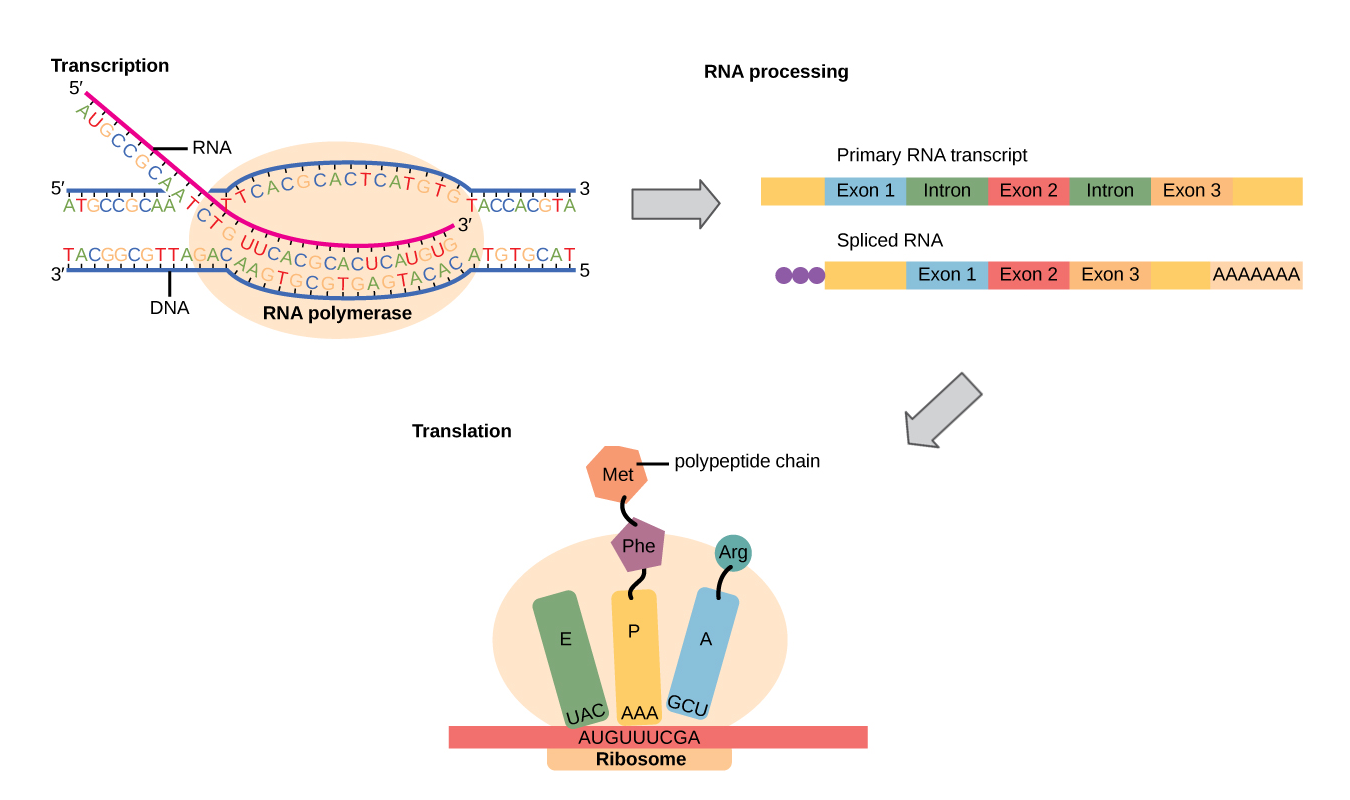
\includegraphics[scale=0.35]{documents/latex/figures/1/dogma.png}
    \caption{Transferencia de la información genética. El ADN es transcripto en forma de ARN (ARN mensajero). Luego el ARN mensajero es ``cortado'' uniendo los exones (partes codificantes del gen) en un proceso denominado \textit{splicing}. Por último, los ribosomas usan la información para unir los aminoácidos en forma de proteína. Imagen tomada de OpenStax \cite{OpenStaxCNX}.}
    \label{fig:esquema_dogma}
\end{figure}


\begin{figure}[H]
\centering
    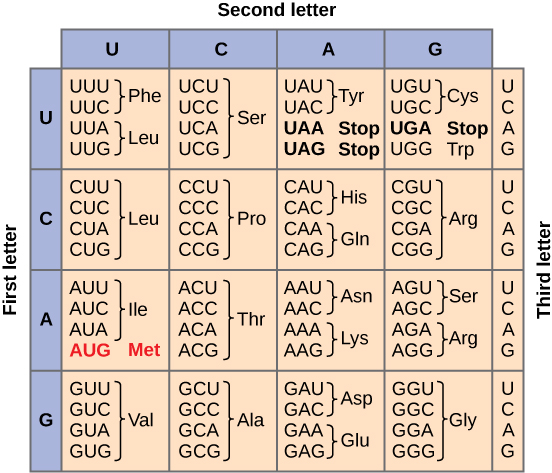
\includegraphics[scale=0.8]{documents/latex/figures/1/tableCodon.jpg}
    \caption{Tabla de codones para generar un determinado aminoácido o símbolo de terminación (\textit{Stop}). Imagen tomada de OpenStax \cite{OpenStaxCNX}.}
    \label{fig:table_codon}
\end{figure}

\newpage


\subsubsection{Variaciones genéticas}

Las variaciones genéticas son diferencias en el ADN entre individuos de una población \cite{EMBL}. Estas variaciones pueden ser causadas por mutaciones en el momento de la replicación del material genético, siendo éstas de carácter permanente. Las mutaciones genéticas representan un porcentaje muy pequeño con respecto a la secuencia completa del genoma (alrededor del 0.5\%), pero muchas de ellas son responsables de variaciones fenotípicas, es decir, nuestros rasgos ``observables''. 

Estas variaciones se dividen en tres grupos principales:

\begin{itemize}
    \item Polimorfismos de un sólo nucleotido (SNPs): sustitución de un único par de bases. 
    \item Inserciones o deleciones (indels): pueden ocurrir en un intervalo grande del ADN de entre 2 a 200 pares de bases.
    \item Variaciones estructurales: ocurren en secuencias largas de bases, y pueden ser indels, inversiones, duplicaciones, entre otras.
    
\end{itemize}

Finalmente, cualquiera de estas variaciones pueden ser beneficiosas para el organismo, neutrales (sin efecto alguno) o perjudiciales. 

\subsubsection{Polimorfismos de un sólo nucleótido}

En el marco de esta tesis estudiaremos los polimorfismos de un sólo nucleótido, o SNPs por sus siglas en inglés (Single Nucleotide Polymorphism). 

En la figura \todo{X} podemos ver los distintos tipos de SNP. De acuerdo al lugar, pueden ocurrir en una zona codificante, es decir una porción del gen que codifica una proteína, o en una zona no codificante, como los intrones (partes del gen no codificante).

Dentro de las sustituciones en la zona codificante, algunas mutaciones pueden ser sinónimas, es decir que existe un cambio en uno de los nucleótidos del ADN pero dicho nucleótido es reemplazado por uno igual. También puede ocurrir una sustitución no sinónima, en donde el nucleótido es reemplazado por uno distinto. Esto no necesariamente genera un cambio en el aminoácido que lo codifica. Podemos ver en la tabla \ref{fig:table_codon} que el muchos codones codifican el mismo aminoácido, por ejemplo, los codones AAU, AUC y AUA codifican el aminoácido isoleucina. Luego, si en la cadena de ADN, el codón AUA sufre una mutación en su último nucleótido, pasando a ser AUC, dicho codón seguirá codificando para el mismo aminoácido (ver tabla \ref{fig:table_codon}). Estas sustituciones se denominan sustituciones no sinónimas silenciosas (\textit{silent}).

En particular estudiaremos los SNPs con cambio de sentido (\textit{missense}), es decir aquellos que deriven en un cambio de aminoácido en la proteína producida por la variante del gen. \textbf{El problema que intentaremos atacar es detectar aquellos SNPs cuyo cambio en el aminoácido de la proteína generada pueda estar asociado a alguna patogénesis}. 


% \subsubsection{Las enfermedades poco frecuentes (EPOF)}

% \subsubsection{\todo{TODO}}

\section{Enfoque computacional}

Para atacar este problema, decidimos usar métodos de aprendizaje automático. El aprendizaje automático es un método computacional (dentro del área de la inteligencia artificial y la estadística) que consiste en aprender a partir de los datos. 

Utilizamos este enfoque en particular dado que es el que utilizan los trabajos que se realizan en este área. La principal ventaja es la gran cantidad de efectos conocidos de las variantes proteicas, y a su vez la ubicación (\textit{locus}) en el genoma. Estos datos se encuentran (en gran parte) de forma abierta y gratuita. Usando esta fuente de datos intentaremos entrenar un modelo que pueda predecir con un cierto grado de precisión el efecto de una variante no estudiada. 

Existen diferentes formas de categorizar los algoritmos de aprendizaje automático. Una de las formas posibles es la categorización de acuerdo a la cantidad de tipo de supervisión durante la fase de entrenamiento. Este aprendizaje puede ser \cite{Barber2011}:

\begin{itemize}
\item Supervisado, en donde se utilizan ejemplos previos que están ``rotulados'', es decir que posee una variable de respuesta conocida y se busca conseguir una predicción lo más certera posible sobre nuevos datos. 
\item No supervisado, donde el objetivo es encontrar distintos grupos o clusters dentro de los datos.
\item Semi-supervisado, en el que se trabaja con un pequeño conjunto de datos etiquetados y un conjunto mucho mayor de datos no etiquetados. El objetivo está en usar este último conjunto para mejorar el clasificador construido con los datos etiquetados.
\item Por refuerzo, donde un \textit{agente} observa el entorno y realiza diferentes acciones para maximizar la recompensa. El modelo a aprender entonces es la estrategia que le permite tomar decisiones ante determinadas situaciones. 
\end{itemize}

En este trabajo nos vamos a centrar exclusivamente en el tipo de aprendizaje supervisado.

\subsubsection{Aprendizaje supervisado}

Como mencionamos anteriormente, el aprendizaje supervisado trata de predecir una respuesta usando un modelo generado con datos correctamente etiquetados. Definido de manera formal, dado un set de datos $ \mathcal{D} = \{(x^n, y^n), n = 1...N\}$  buscamos aprender la relación entre el ejemplo $x$ y la variable de respuesta $y$ tal que al recibir un nuevo ejemplo $x^*$ la respuesta predicha $y^*$ sea precisa \cite{Barber2011}. La precisión está definida formalmente por la función de pérdida o \textit{Loss Function}, $L(y^{pred}, y^{true})$. Esta función nos permite medir el costo de errar en la predicción y por lo tanto cuantificar qué tan bueno es nuestro modelo. A continuación haremos un recorrido por los métodos que usamos en esta tesis.

\subsubsection{Regresión logística}

La regresión logística (LR) es un modelo basado en la regresión lineal. Al igual que este, consiste en buscar los coeficientes de una función de manera que la \textit{loss function} de la función sea el mínimo. A diferencia de la regresión lineal, que usa una función lineal (o polinomial) para aproximar los puntos (que son valores continuos), la regresión logística usa la función logística para aproximar los valores (que son categóricos). Esta función, generalizada para multiples variables predictoras y variable de respuesta binaria se define como:

\begin{equation*}
h_{\theta}(\boldsymbol{X}) = \frac{1}{1 + e^{\theta^{T}\boldsymbol{X}}} = Pr(Y = 1 | \boldsymbol{X}; \theta)
\end{equation*}

donde $\boldsymbol{X}$ representa el vector de variables predictoras, $\theta$ es el vector de coeficientes y $Y$ es la variable de respuesta. Lo que se busca modelar, es la probabilidad de pertenecer a una clase determinada (simbolizada con '1'), dado que las variables observadas son $\boldsymbol{X}$ y usando los parámetros $\theta$. Los parámetros $\theta$ son obtenidos buscando maximizar la verosimilitud con los parámetros de la distribución real de los datos \cite{Hastie2001}. La probabilidad de pertenecer a la otra clase entonces, es igual a 1 - $h_{\theta}(\boldsymbol{X})$.

\subsubsection{Support Vector Machines}

Las Support Vector Machines (SVM) son al igual que la regresión logística, métodos lineales de clasificación. Esto significa que también busca una frontera de decisión (\textit{decision boundary}) que define la clase a la que pertenecen los datos. En este caso no se busca hallar los parámetros de la distribución a modelar sino que el objetivo reside en encontrar el hiperplano (o \textit{Support Vector}) que mejor separe a los datos de entrenamiento. 

\subsubsection{Random Forest}

A diferencia de los algoritmos anteriores, Random Forest esta basado en un método de clasificación basado en árboles de decisión. Estos métodos se caracterizan por segmentar el espacio de predicción en un número de regiones. Para entender Random Forest, resulta muy útil conocer el funcionamiento de los árboles de decisión. 

Un árbol de decisión se construye dividiendo el espacio de variables de forma recursiva, recorriendo la lista de variables y seleccionando la variable que mejor divide las clases de acuerdo a un criterio determinado. El criterio que decidimos usar en este trabajo, por ser el más usado en tareas de clasificación, es el índice Gini (también referido como pureza):

\begin{equation*}
    G = \sum_{k = 1}^{K} \hat{p}_{mk}(1 - \hat{p}_{mk})
\end{equation*}

donde $\hat{p}_{mk}$ representa la proporción de la clase $k$ en la región $m$. Uno de los principales problemas que presenta este enfoque es la alta varianza (\textit{variance}) con respecto a los datos de entrenamiento. Si la profundidad del árbol es muy grande, aumenta el riesgo de \textit{overfitting} en los datos que poseemos. 

En el caso de Random Forest, se construyen distintos árboles de decisión con subconjuntos escogidos de forma aleatoria, con el objetivo de disminuir la varianza. A la vez, al ser árboles de poca profundidad (que favorecen el \textit{underfitting}), se genera una cantidad alta de árboles para solucionar el problema de alto sesgo (\textit{bias}).

Una de las principales ventajas de Random Forest es su interpretabilidad. Esto se expresa en la posibilidad de calcular fácilmente la importancia de las variables en el modelo. La importancia de una variable (o \textit{feature importance}) se calcula como el promedio del índice Gini en cada uno de los nodos de los árboles donde aparece, expresada proporcionalmente a la importancia máxima de todas las variables \cite{Hastie2001}.  

% \subsubsection{Pipeline de entrenamiento y evaluación}

% Cada uno de estos métodos involucran una fase de entrenamiento en donde se genera la función de decisión del modelo. En nuestro trabajo la fase de entrenamiento consta de 

\subsubsection{Métricas de evaluación}

Las medidas son las siguientes:

\begin{itemize}
    \item \textbf{Precisión}: La Precisión del modelo, está medida como la cantidad de positivos correctamente calificados (verdaderos positivos) sobre la cantidad de instancias calificadas como positivas (verdaderos positivos y falsos positivos).
    
    \begin{equation*}
        \frac{VP}{VP + FP}
    \end{equation*}
    
% \pagebreak
    \item \textbf{Recall}: El Recall corresponde a la cantidad de verdaderos positivos sobre el total de positivos (verdaderos positivos y falsos negativos).
    
    \begin{equation*}
        \frac{VP}{VP + FN}
    \end{equation*}
    
    \item \textbf{F1-Score}: El F1-Score es el promedio armónico entre la Precisión y el Recall. Usamos el promedio armónico de manera de afectar negativamente el resultado si alguno de los valores es especialmente bajo. Posee un rango de 0 a 1. 
    
    \begin{equation*}
        F_1 = \frac{2}{\tfrac{1}{\mathrm{recall}} + \tfrac{1}{\mathrm{precision}}} = 2 \cdot \frac{\mathrm{precision} \cdot \mathrm{recall}}{\mathrm{precision} + \mathrm{recall}}
    \end{equation*}
    
\end{itemize}

\section{Trabajos relacionados}

\subsubsection{VarQ \cite{Radusky2017}}

VarQ es una herramienta generada en el BIA (Plataforma Bioinformática Argentina) por Leandro Radusky. Esta herramienta permite extraer datos estructurales de variantes proteicas de un sólo aminoácido (SAS, por sus siglas en inglés) tomando información de diferentes bases de datos o aplicaciones (PDB, PFam, 3DID, entre otras), permitiendo el análisis manual de los diferentes cambios estructurales, como el tipo de actividad, el plegamiento, si pertenece a un sitio activo, o si forma parte en interfaces proteína-proteína. 

\begin{figure}[H]
    \centering
    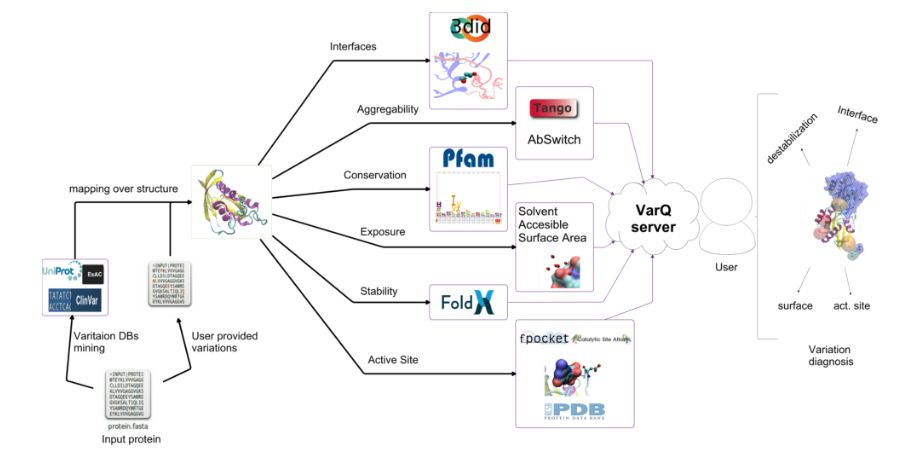
\includegraphics[scale=0.4]{documents/latex/figures/1/pipeline.png}
    \caption{Pipeline de extracción de datos de la herramienta VarQ. Esta figura fue extraída de la tesis de doctorado de Leandro Radusky.}
    \label{fig:varq_pipeline}
\end{figure}

En la primera parte de esta tesis hacemos uso del trabajo de Santiago Moreno. Uno de sus objetivos principales de fue generar un dataset de variantes a nivel de proteínas (dataset VarQ), y evaluar la performance de un modelo que predice el efecto de la mutación usando las variables que provee esta herramienta. 

\subsubsection{VEST \cite{Carter2013}}

VEST (\textit{Variant Effect Scoring Tool}) es un predictor de efectos funcionales de SNPs con cambio de sentido (en regiones codificantes) desarrollado en el Karchin Lab de la Universidad de Johns Hopkins. Con esta herramienta (basada en Random Forest) analizaron aproximadamente 80,000 variantes anotadas de HGMD (\textit{Human Gene Mutation Database}) con variables de tipo genómicas, estructurales y físico-químicas.

\subsubsection{FATHMM-MKL \cite{Shihab2015}}

FATHMM-MKL (\textit{Functional Analysis through Hidden Markov Models}) es también un predictor de efectos funcionales de SNPs con cambio de sentido, en regiones codificantes y no codificantes. Fue desarrollado en la Universidad de Bristol. Proponen un método integrador combinando los scores de diferentes predictores (entre ellos VEST).

% \newpage


\section{Objetivos y estructura del trabajo}

El objetivo del trabajo se centra en responder una serie de interrogantes generados a partir del estudio de los trabajos previos:

\begin{itemize}
    \item El dataset de VarQ se concentra en variables de tipo estructural. ¿Podemos enriquecerlo con variables de otras dimensiones (físico-químicas, genómicas, filogenéticas)?
    \item ¿Cómo afectan las distintas variables a nuestros modelos? ¿Cuáles son las más importantes?
    \item ¿Cuáles son los mejores algoritmos de aprendizaje automático para resolver este tipo de problemas y cuáles son sus parámetros?
    
\end{itemize}

Intentaremos responder estas preguntas en este trabajo, que se encuentra dividido en 5 partes principales:

\begin{itemize}
    \item Modelo usando el dataset VarQ
    \item Modelo usando propiedades físico-químicas de la proteína
    \item Modelo usando variables genómicas
    \item Integración de propiedades fisico-químicas y variables genómicas
    \item Modelo generado con el dataset VarQ y el dataset Integral.
\end{itemize}


